\section{ (30 pts)}
For a bivariate random variable $X = (X_1, X_2)$ with the following unnormalized \textsc{pdf}:
\begin{equation*}
	\hat{f}_X(x_1, x_2) = \exp \left(-\left(x_1 - \frac{x_2^2}{4}\right)^2 - \frac{x_2^2}{4}\right)
\end{equation*}
Using a sample random walk Gaussian distribution $q(x'|x)$ as our proposal
\begin{equation*}
	q(x'|x) = \mathcal{N}(x';x,\sigma^2 I)
\end{equation*}
where we fix $\sigma = 0.2$, we are going to implement a Metropolis-Hastings algorithm based Markov-Chain Monte-Carlo sampler for the target distribution $\hat{f}_X(x_1,x_2)$. 
To do so, first, we draw the contour plot of the density. 
Next, we implement the algorithm to run the random walk Metropolis-Hastings, and finally, we verify the correctness of our implementation by visualizing samples provided.
The code is as follows:
\begin{lstlisting}[language=Python]
# x: n times 2 matrix or 2 dimensional vector
def log_f_tilde(x):
	if x.ndim == 2:
		x1, x2 = x[:,0], x[:,1]
	else:
		x1, x2 = x

	return -(x2 - x1**2/4)**2 - x1**2/4

def plot_density(alpha=1.0):
	nx, ny = 50, 50
	x = np.linspace(-5, 5, nx)
	y = np.linspace(-2, 4, ny)
	xx, yy = np.meshgrid(x, y)
	z = np.exp(log_f_tilde(np.concatenate([xx.reshape((-1, 1)), 
	yy.reshape((-1, 1))], -1)))
	plt.contour(x, y, z.reshape((nx, ny)), cmap='inferno', alpha=alpha)

plot_density()

# propose a sample from the proposal distribution q(x' | x) = N(x' ; x, sigma^2*I)
def q_MH(x, sigma):
	# Sample epsilon_1, epsilon_2 ~ N(0,1)
	epsilon = npr.normal(0, 1, x.size)
	# Sample x_acc ~ N(x, sigma^2*I)
	x_acc = x + sigma*epsilon
	return x_acc

# run a random-walk Metropolis Hastings
# x0: initial sample
# num_samples: number of samples to collect
# sigma: variance for the proposal distribution
def RW_MH(x0, num_samples, sigma):
	x = np.expand_dims(x0, axis=0)
	for i in range(1, num_samples):
		x_i = x[-1,:]
		# Generate x_acc from q_MH
		x_acc = q_MH(x_i, sigma)
		# Compute Accptance Probability
		Acc_Prob = min(1, np.exp(log_f_tilde(x_acc) - log_f_tilde(x_i)))
		# Draw a uniform random number u ~ U(0,1)
		u = npr.rand(1)
		# Accept if u <= Acc_Prob, Reject otherwise
		if u <= Acc_Prob: 
			x = np.append(x, np.expand_dims(x_acc, axis=0), axis=0)
		else: 
			x = np.append(x, np.expand_dims(x_i, axis=0), axis=0)
	return x

# randomly initialize a chain
x0 = 0.01*npr.randn(2)
# collect 10000 samples from RW MH
x = RW_MH(x0, 10000, 0.2)

# visualize the samples
plot_density(alpha=1.0)
plt.scatter(x[:,0], x[:,1], alpha=0.1, color='b')
\end{lstlisting}
Here are the results we obtained while executing the code.
\begin{figure}[h]
	\centering
	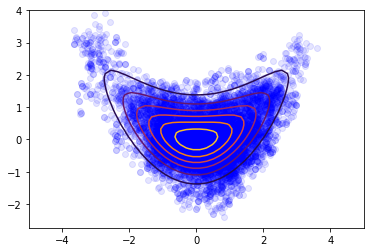
\includegraphics[width=.4\textwidth]{4.png}
\end{figure}
Since the contained samples are distributed tightly around the contour plot, it can be verified that our algorithm works properly.